As a first example problem, we will consider structural compliance and the method given in \cite{andreassen_clausen_schevenels_lazarov_sigmund_2010}.
A Julia implementation of the code may be found in the appendices.

The MBB beam is a classic problem from mechanical engineering for topology optimization. Within $\Omega$,
subject to natural constraints on cost and area, we would like to build a maximally stiff structure.
Intuition would serve a solution with stacked triangles, as will be observed.

\begin{figure}
    \centering
    \caption{$\Omega$ for \texttt{top88.jl} with the applied boundary conditions and loads.}
    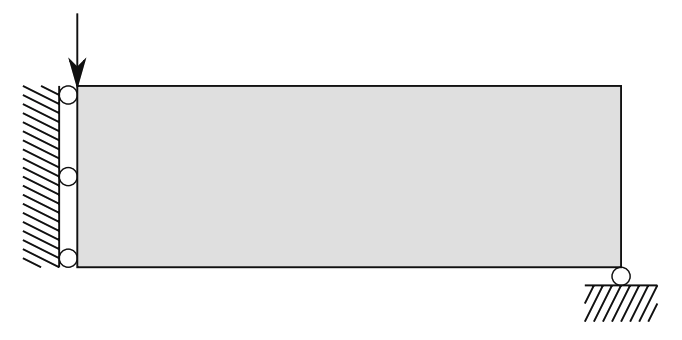
\includegraphics[width=\textwidth]{imgs/Top88/problem_diagram.png}
\end{figure}

\subsection{Problem Specification}

The domain $\Omega$ is discretized with (square) quadrilateral elements and the density approach is adopted,
so, to each element $e$ in the domain, we will associate a material density $x_e$ that is used to determine
its Young's modulus $E_e$ by
\begin{equation}
    E_e(x_e) = E_{\text{min}} + x_e^p (E_0 - E_{\text{min}}).
\end{equation}
As mentioned, $p$ is typically taken to be $3$ and $E_{\text{min}}$ is a relatively very small value
that is assigned to all elements for primarily numerical reasons -- in particular, we avoid running into
a singualr stiffness matrix. \cite{andreassen_clausen_schevenels_lazarov_sigmund_2010} titles this a
``modified SIMP approach.'' Following the format of \autoref{eq:general_continuous}, the problem may be
written
\begin{equation}\label{eq:top88_problem}
    \begin{aligned}
        \min_{\mathbf{x}} &\quad c(\mathbf{x}) := U^T K U = \sum E_e(x_e) u_e^T k_0 u_e\\
        \text{s.t.} &\quad V(x)/ V_0 = \theta,\\
            &\quad KU = F,\\
            &\quad 0 \leq \rho \leq 1.
    \end{aligned}
\end{equation}
Here, $c$ defines the compliance, $U$ and $F$ denote resp. the global displacement and force vectors, $K$
is the global stiffness matrix, $u_e$ is the element displacement vector, $k_0$ is the element stiffness
matrix (for a unit Young's modulus), and $\mathbf{x}$ denotes the element densities/ material distribution.
Lastly, $V(x)$ denotes the volume of $x$, $V_0$ of the entire domain $\Omega$, and $\theta$ is a prescribed
volume fraction (ie, the fraction of the design domain the structure is allowed to take up).

\subsubsection{Optimality Criteria Method}

The optimization problem is solved with a standard optimality criteria method.
\begin{equation}
    x_e^{t+1} = \begin{cases}
        \max(0, x_e - m) & \text{if } x_e B_e^\eta \leq \max(0, x_e - m)\\
        \min(1, x_e + m) & \text{if } x_e B_e^\eta \geq \min(1, x_e + m)\\
        x_e B_e^\eta & \text{otherwise.}
    \end{cases}
\end{equation}
$m$ is a positive move limit, $\eta (= 1/2)$ is a numerical damping coefficient, and $B_e$ is obtained
from the optimality condition as
\begin{equation}
    B_e = \frac{-\frac{\partial c}{\partial x_e}}{\lambda \frac{\partial V}{\partial x_e}},
\end{equation}
where the Lagrangian multiplier $\lambda$ must be chosen such that the volume constraint is satisfied, which
can be found with a bisection algorithm.

The partials of the objective function $c$ and material volume $V$ with respect to $x_e$ are
\begin{equation}
    \frac{\partial c}{\partial x_e} = -p x_e^{p-1} (E_0 - E_{\text{min}}) u_e^T k_0 u,
\end{equation}
and
\begin{equation}
    \frac{\partial V}{\partial x_e} = 1,
\end{equation}
which comes from the assumption that each element has unit volume (so, observe that a decrease in density at
one element will lead to an equal increase in density at another element such that the volume of the structure
overall has not shifted).

\subsubsection{Filtering}

The code implements both a density and a sensitivity filter, and the filtered densities are output.

\subsection{Result}

Confirming roughly our intuition, we see a number of triangles forming. The following was run on a rectangle
of 150x50 elements with a volume fraction of $0.5$, $r_{\text{min}} / V(e) = 2.0$ (ie, radius divided by element volume),
and using a density filter.

\begin{figure}[H]
    \centering
    \caption{\texttt{top88} solution on 150x50 rectangle.}
    
\includegraphics[width=\textwidth]{imgs/Top88/r150x50_density.png}
\end{figure}